This chapter provides an overview over current blockchain applications in field of logistics and supply chain management both in academia and industry. Through analyzing the performance, feedback, research, it helps us prepare for the next implementing step. Last but not least, I will present the preparation for setting up the application, especially the consideration on how to choose the right platform.

\section{Research in the Scientific Community}
Since 2017 the amount of research papers discussing the possibility of applying blockchain technologies into logistics field have witnessed a sudden blowout. It draws great attention from academical world. 

In 2017, Finnish researchers haven dived into the integration blockchain into Digital Supply Chain (DSC), they pointed out that traditional integration of DSC seemed to be a significant gap in many functionalities. This was an interesting finding, as intermediates (EDI operators)including banks (SWIFT operators) have been operating and collaborating in this area over two
decades, but services still lack some fundamental
functionalities (e.g. standards, timestamping of
transactions, monitoring and tracking of information
flows and secure end-to-end delivery of information).An analysis showed many of these missing
functionalities to be embedded in blockchain technology.\cite{chapter4-dsc}

Researchers from China attempt to address the agri-food safety problem through optimizing the food supply chain. They depicted a system using RFID and blockchain technology in building the agri-food supply chain traceability system, including production link, processing link, warehousing management link, cold chain distribution link, Sales link. When consumers are shopping in the supermarket, they can use the
RFTD reader to obtain the basic infonnation of agri-food
products by scanning their RFID tags. All the information along the agri-food supply chain is fully realtime auditable in blockchain.
Transparency of products information could significantly
enhance the consumers' trust for products and obviously
increase their confidence for the agri-food markets.\cite{chapter4-RFID}

Remarkably researchers from Portland University proposed a block-supply
chain, a new decentralized supply chain that detects counterfeiting
attacks using blockchain and Near Field Communication (NFC). Their simulations show that the proposed protocol offers remarkable performance with a satisfactory level of security compared to the state of the art consensus protocol Tendermint.\cite{chapter4-nfc}

\section{Trial in Industry}
From any perspective, the industry field is always the first one to perceive the great potential and chance laying in blockchain.
Indeed some enterprises are actively trying out the exploration. There we can have a look at the those applications from different perspective.

\subsection{Classification}
There exists several criteria can be used to classify blockchain applications. Therefore we try to list the as complete critertia as we can to provide better view of the applications.
\subsection{Products or Platforms}
Blockchain applications can be categorized into two camps: product-oriented or platform-oriented. The distinct also shows in the the business models they run. The product-oriented applications is B2C model which provides clients the blockchain-based solution in specific scenarios. The example are like uPort mentioned in the previous chapters, controls the users' ownership of identity. Another type is the
platform-oriented, which is more familiar to most of blokchain developers. The second type usually provides open sourced platform, aiming to setup the field standard, and gradually to build a ecosystem. Hyperledger Fabric and Corda are the latter type, which have wilder ambitions.

\subsubsection{Assets and Token}
First and most of second generation of blockchains like Bitcoin or Ethereum, have native tokens (or Cryptographic Tokens, Cryptocurrency). 
Token are part of the incentive scheme to encourage a disparate group of people who do not know or trust each other organize themselves around the purpose of a specific blockchain. And the new generation of blockchain like Corda and Hyperledger were designed to run with a single shared ledger among all network participants. This allows any participant to view all transactions, including those of competitors. While smart contracts provide an amazing leap forward in how blockchain can be applied to business transactions. 
%(blockchain ubiquity)
\subsubsection{Consensus Algorithms}
The Consensus algorithm has vast effect on blockchain systems' features. Especially the performance, whether it has mining process or not is the key issue. In chapter 2, we gave a precise introduction and comparison of consensus algorithms. The table will help readers to categorize the applications. 

\subsubsection{Business Scope}
While we described above the blockchain applications from a technology perspective, we can also use a commercial approach to map them. Since in different fields of usage, the requirement for security level, running platform, scalability,etc will be distinguishing. Also in the end of Chapter 2, we listed out a wide variety of applications in all kinds of areas.
\subsubsection{Open or Close Source}
For most of open source projects, their incentives are to provide a standard platform, which ultimately to create a ecosystem. And some close source projects attempt to protect the intellectual property, which sell the projects as product. This prospective of categorization is similar to the first one we mentioned above.
\subsection{Platform Benchmarks Overview}
Blockchain technology is recently under extensive research and development,
leading to a high market fragmentation. Until November 2018, according to incomplete statistics, there exists more than one hundred blockchain projects\cite{platforms}, we list the top 5 popular platforms with detailed description, also the Table 5.1 compares the key characteristics of the mature platforms. 

\begin{itemize}
	\item Ethereum \\
	Mature Smart Contracting Cross-Industry Platform. Ethereum Wallet that allows holding crypto-assets, and writing, deploying and using smart contracts. Making cryptocurrencies. Theoretically speaking, it is a generic platform for all kinds of transactions and applications. Concurrently it has obvious limitations ans shortness. It is PoW based which is not the fastest (resulting in potential latency issues) and is a massive energy consumer. Though it might change its consensus algorithm to the fast PoS in future versions.
	\item Hyperledger Fabric\\
	Hosted by Linux Foundation and launched in 2016, is an open-source collaborative effort to advance cross-industry blockchain technologies. One of its key goals is to create enterprise-grade distributed ledger frameworks and codebases. Hyperledger Fabric provides a modular architecture, which allows components 
	such as consensus and membership services to be plug-and-play. Hyperledger Fabric 
	leverages container technology to host smart contracts called "chaincode" that comprise 
	the application logic of the system
	\item Quorum\\
	An open source private Blockchain network developed by JP Morgan from the 
	Ethereum code. Quorum’s essential distinguishing feature is the fact that it allows private transactions between the parties. Ideal for applications requiring high speed and throughput processing of private transactions.  It does not use the Proof of Work (PoW) consensus algorithm but uses vote-based and other algorithms enabling it to process hundreds of transactions per second, depending on how smart contracts and networks are configured. 
	\item Corda\\
	R3 is a consortium of some of the world's biggest financial institutions that has created an open-source distributed ledger platform called Corda. A distributed ledger platform Like Hyperledger Fabric, it is a product designed from the ground up for enterprise networks, generally banks, finance. There is no built-in token or cryptocurrency for Corda, and it is a permissioned blockchain as it restricts access to data within an agreement to only those explicitly entitled to it, rather than the entire network. Its consensus system takes into account the reality of managing complex financial agreements. It is also known for its focus on interoperability ease of integration with legacy systems.  
	\item BigChainDB\\
	An open source system
	 that starts with a big data distributed database and then adds Blockchain characteristics - decentralized control, immutability and the transfer of digital assets. It focuses on the distributed database, so here we exclude BigChainDB from our project of development.
\end{itemize}
\begin{landscape}% Landscape page
	\thispagestyle{empty}% empty page style (?)
	%\centering % Center table

	\begin{table}[H] \centering 
		%	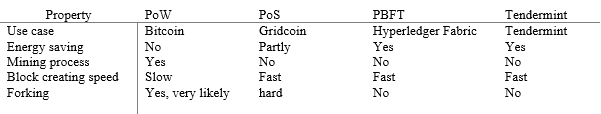
\includegraphics[scale=0.9]{charts/consensus}
		\ra{1.2}

		\begin{tabular}{{m}{3.5cm}cM{2.5cm}M{2.7cm}M{2cm}{m}{1.8cm}ccc}
		\toprule[0.6mm]
			Projects & Start year & Governance  & Popularity
			(GitHub stars)& Smart Contract & Consensus&Throughput &	VM&Oracle\\ 
			\midrule[0.3mm]
			
			Ethereum & 2015	&Ethereum Foundation& 21k&	Yes &PoW&15 tps& EVM&Yes\\
			
			Quorum & 2013&J.P.Morgan&2799&Yes& Voting&10+ to 100+ tps&EVM&-\\
			
			Hyperledger Fabric & 2016&IBM&7280 &Yes&PBFT& > 2000 tps& Docker&No\\
			
			Corda& 2015& R3 &2519& Yes& pluggable&~ 170 tps	&JVM&Yes\\
			
			BigChainDB&2013	& BigChainDB& 2992&	No&	Tendermint&N/A &Optional&Yes\\ 
			Monax &2014	&Monax&271&Yes&Tendermint&N/A&EVM&No\\
			Multichain&2015	&Coin Sciences	&441&No&PBFT,round robin, etc&100-1000 tps&No&No\\
			Ripple&2014&Ripple Labs&3k&	No&	Probabilistic Voting&0.25 tps&RVM&No\\
			
			\bottomrule[0.5mm]
		\end{tabular}

	\caption{Comparison of different blockchain platforms}
	\end{table}
\end{landscape}

\begin{comment}
\begin{landscape}% Landscape page
	\thispagestyle{empty}% empty page style (?)
	%\centering % Center table
	\begin{figure}\centering% order of placement preference: here, top, bottom
		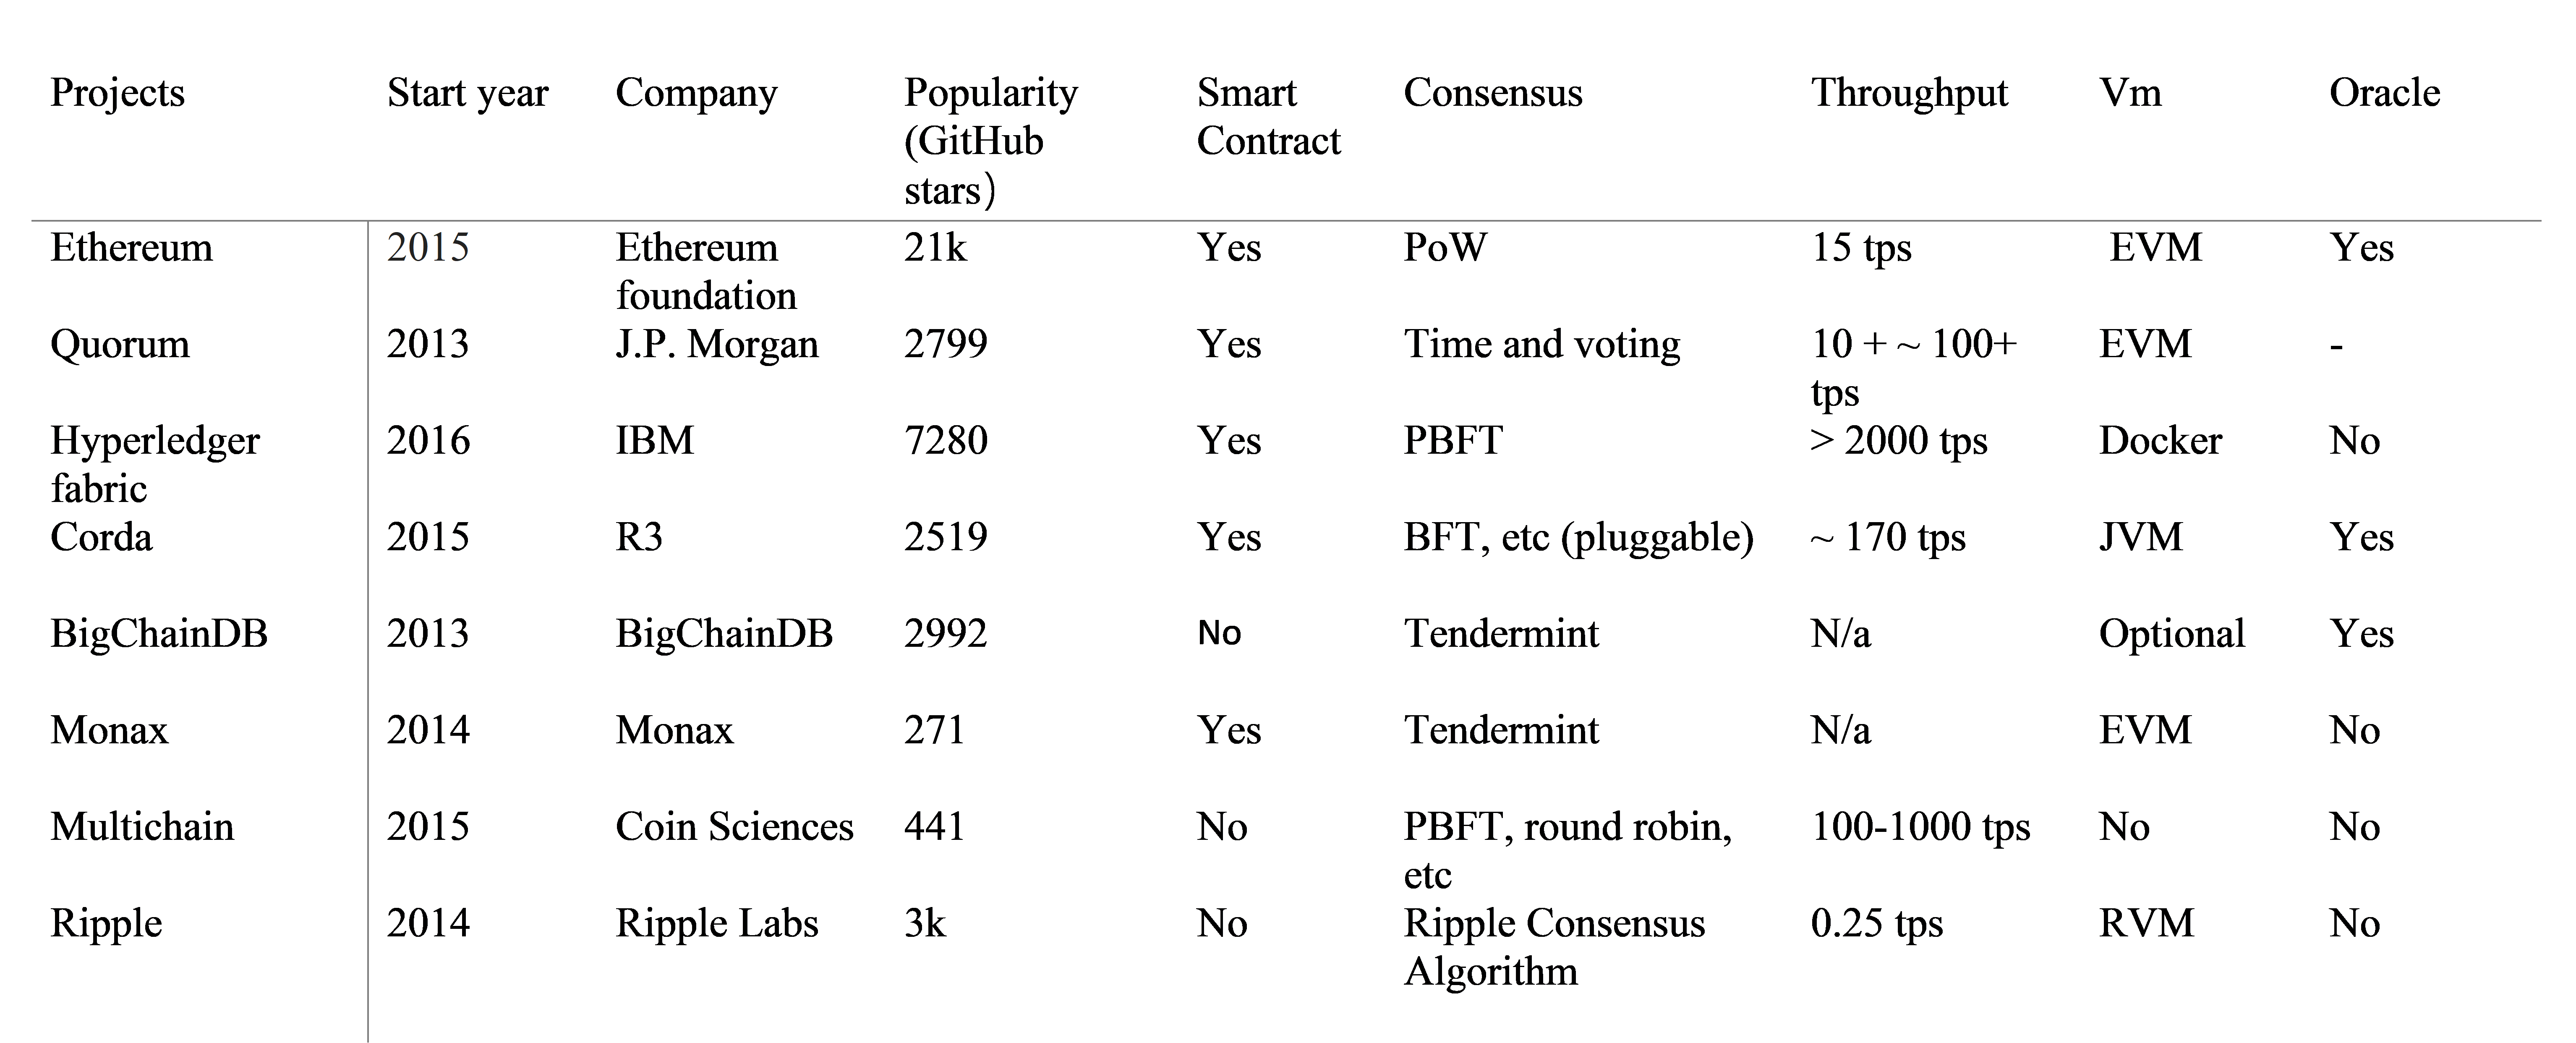
\includegraphics[scale = 0.23]{charts/benchmark}
		\caption{Comparison of different blockchain platform}
	\end{figure}
\end{landscape}
\end{comment}
\clearpage

\subsection{Criteria for platform selection}
As fully described and compared above, there are multitude of different blockchain platforms with specific functional incentives. How to choose the proper platform without getting overwhelmed in the sheer volume of potential techniques? Researchers from Fraunhofer FIT gave a set of criteria\cite{fraunhofer} for selecting the right one:
\begin{itemize}
	\item Access policy – Permissioned vs. public blockchain;\\
	In our case, considering the industrial confidentiality, permissioned platform is required, thus the Ethereum will not be taken into consideration.
	\item Process integration – Availability of smart contracts or
	chain code;\\
	Some projects provides a network for their native cryptocurrency, like Ripple and Multichain are not suitable here.  
	\item Scalability and transaction performance – Transaction
	throughput;\\
	This is extremely important in the industrial cases. In blockchain systems, we use "transaction per second (tps)" as the measurement for performance.
	\item Restricting data access – Data privacy and visibility;\\
	The first and part of second generations of blockchain, like Ethereum, were designed to run with a single shared ledger among all network participants. This allows any participant to view all transactions, including those of competitors. In our scenario,  we prefer platforms like Hyperledger Fabric and Corda which have confidentiality design.
	\item Network governance – Ease of adding/removing nodes
	to the network;\\
	Lightweight administration process should be encouraged, so that the join and exit of the network will not lead to shutdown of the whole system or reconfiguration.
	\item Technology governance – Open source, project
	management, development kits.\\
	The last criterion is also of major importance, because the technology governance will vastly impact your project's performance, stability, development process and success. Especially for open source project, 
	developers should better examine whether the future of the platform is guaranteed, i.e. whether the it is periodically and stably updated, whether the bugs are solved in time, etc

\end{itemize}
In sum, for the Turnover Box System, we need a permissioned blockchain framework, with usable and efficient method for digital asset, smart contract development. Hyperledger Fabric, R3 Corda, Quorum are all qualified open source options, however considering the unstable throughput of Quorum, we narrows the options only to the Hyperledger Fabric and Corda.

\subsubsection{Hyperledger Fabric vs. Corda}
\begin{outline}
	\1 Languages Support
		\2 Fabric support for: 
			\3 Go(since v1.0)
			\3 Node.js(since v1.1)
			\3 Java(since v1.3)
		\2 Corda support Java and Kotlin
	\1 Prerequisites for development
		\2 Fabric requires the tools to be installed:\\ 
			1. cURL\\
			2. Docker and Docker Compose\\
			3. Go version 1.10.x is required\\
			4. Node.js Runtime and NPM\\
			5. Python for Ubuntu 16.04 users\\
		\2 Corda uses industry-standard tools: \\
			1. Oracle JDK 8 JVM - minimum supported version 8u171\\
		    2. IntelliJ IDEA - supported versions 2017.x and 2018.x\\
		    3. Git\\
	\1 Database and Queryability
		\2 Fabric has a state database based on either \textbf{LevelDB} or \textbf{CouchDB}, both support key range queries
		\2 Corda uses a relational database for data storage, supports SQL  including H2, SQLServer, and PostgreSQL, can be direct accessed.
	\1 Platform support
		\2 Fabric supports most of the OS and architectures. And major cloud providers have embraced Hyperledger Fabric offerings (AWS, Azure, IBM, Oracle, SAP) 
		\2 Corda runs on the JVM, which can be used widely across different platforms. AWS, Azure are also supported.
     \1 Open Source and Governance
     	\2 Fabric is open source and governed by Linux Foundation. Hyperledger Fabric owns very big community, there are more than 140 contributors and 7000+ stars on Github. 
     	\2 Corda is  also open source governed by company R3. Comparing with Hyperledger, Corda's community is relatively small.
\end{outline}

When consider the developer friendly, precise documentation, performance, etc, it is hard to choose a platform from the two, if we let it remain theoretical. The best way is to try them out, and discuss in the conclusion part.